% \documentclass{beamer}
\documentclass[xcolor=dvipsnames]{beamer}
%% \usefonttheme[onlymath]{serif}
%% \usefonttheme{professionalfonts}
\usefonttheme{serif}
%% \usecolortheme[named=Blue]{structure}
\setbeamersize{text margin left=30mm, text margin right=30mm}
\useoutertheme{infolines}
%% \usetheme[height=7mm]{Rochester}
\usetheme{Pittsburgh}
\setbeamertemplate{items}[ball]
\setbeamertemplate{blocks}[rounded][shadow=true]
\setbeamertemplate{navigation symbols}{}

\usepackage{soul}
\usepackage[utf8x]{inputenc}
%% \usepackage{default}
\usepackage[english]{babel}
\usepackage{geometry}
%% \usepackage{fullpage}
\usepackage{amsmath, amsthm, amssymb}
\usepackage{listings}
\usepackage{pxfonts}
%% \usepackage{color}
%% \usepackage{graphicx}
%% \usepackage{natbib}
%% \usepackage{array}
%% \usepackage{booktabs}
%% \usepackage{tabu}
%% \usepackage[utf8]{inputenc}
%% \usepackage{fancyhdr}
%% \usepackage{float}
%% \usepackage{subfigure}
%% \usepackage{titlesec}

\setbeamertemplate{headline}{}
\setbeamertemplate{footline}[frame number]{}
\setbeamertemplate{navigation symbols}{}
\setbeamertemplate{footline}{}

\renewcommand{\chaptername}{}
\renewcommand{\bibname}{References}
\newcommand{\pluseq}{\:+\!\!=}
\newcommand{\minuseq}{\:-\!\!=}
\newcommand{\mrm}[1]{\mathrm{#1}}
\newcommand{\bsym}[1]{\boldsymbol{#1}}
\newcommand{\abs}[1]{\lvert#1\rvert}
\newcommand{\norm}[1]{\lVert#1\rVert}

\newcommand{\totalderiv}[2]{\frac{\mrm{d} #1}{\mrm{d} #2}}
\newcommand{\partialderiv}[2]{\frac{\partial #1}{\partial #2}}

\newcommand{\totalderivT}[2]{\totalderiv{#1}{#2}^{\mrm{T}}}
\newcommand{\partialderivT}[2]{\partialderiv{#1}{#2}^{\mrm{T}}}


\setcounter{MaxMatrixCols}{20}

\def\CCT{{C\nolinebreak[4]\hspace{-.05em}\raisebox{.4ex}{\tiny\bf ++}}}
\def\CC{{C\nolinebreak[4]\hspace{-.05em}\raisebox{.4ex}{\small\bf ++}}}


\definecolor{lstgray}{gray}{0.93}
\lstset{ %
  escapechar=@,
  language=C++,
  basicstyle=\footnotesize\ttfamily,
  %% basicstyle=\ttfamily,
  %% keywordstyle=\color{blue}\ttfamily,
  keywordstyle=\bfseries,
  stringstyle=\color{red}\ttfamily,
  commentstyle=\color{OliveGreen}\ttfamily,
  morecomment=[l][\color{red}]{\#},
  backgroundcolor=\color{lstgray},
  %% keywordstyle=\color{red},
  frame=f,
  frameround=ffff,
  tabsize=2,
  breaklines=true,
  breakatwhitespace=false,
  showspaces=false,
  showstringspaces=false,
  xleftmargin=5pt,
  xrightmargin=5pt,
  morekeywords={in,out,ref,auto,inout,import,ushort,scope,exit,mixin,decltype,varid,sizeof}
}

\def\redcolor{\color{red}}
\def\bluecolor{\color{blue}}
\def\blackcolor{\color{black}}
\def\graycolor{\color{gray}}
\def\greencolor{\color{OliveGreen}}


\def\sectionname{\translate{Section}}
\def\insertsectionnumber{\arabic{section}}
\setbeamertemplate{section page}
{
  \begin{centering}
    \begin{beamercolorbox}[sep=4pt,center]{part title}
      \usebeamerfont{section title}\insertsection\par
    \end{beamercolorbox}
  \end{centering}
}
\def\sectionpage{\usebeamertemplate*{section page}}


\AtBeginSection{\frame{\sectionpage}}

\usepackage{caption}
\captionsetup[figure]{labelformat=empty}


\title{Philosophical Questions}
\subtitle{University table talk}
\author{Dominic Jones}
\date{June 2018}


\begin{document}
\begin{frame}[plain]
  \titlepage
\end{frame}


\begin{frame}[plain]
\begin{figure}
  \centering
  \begin{columns}
    \column{0.99\textwidth}
    \centering
    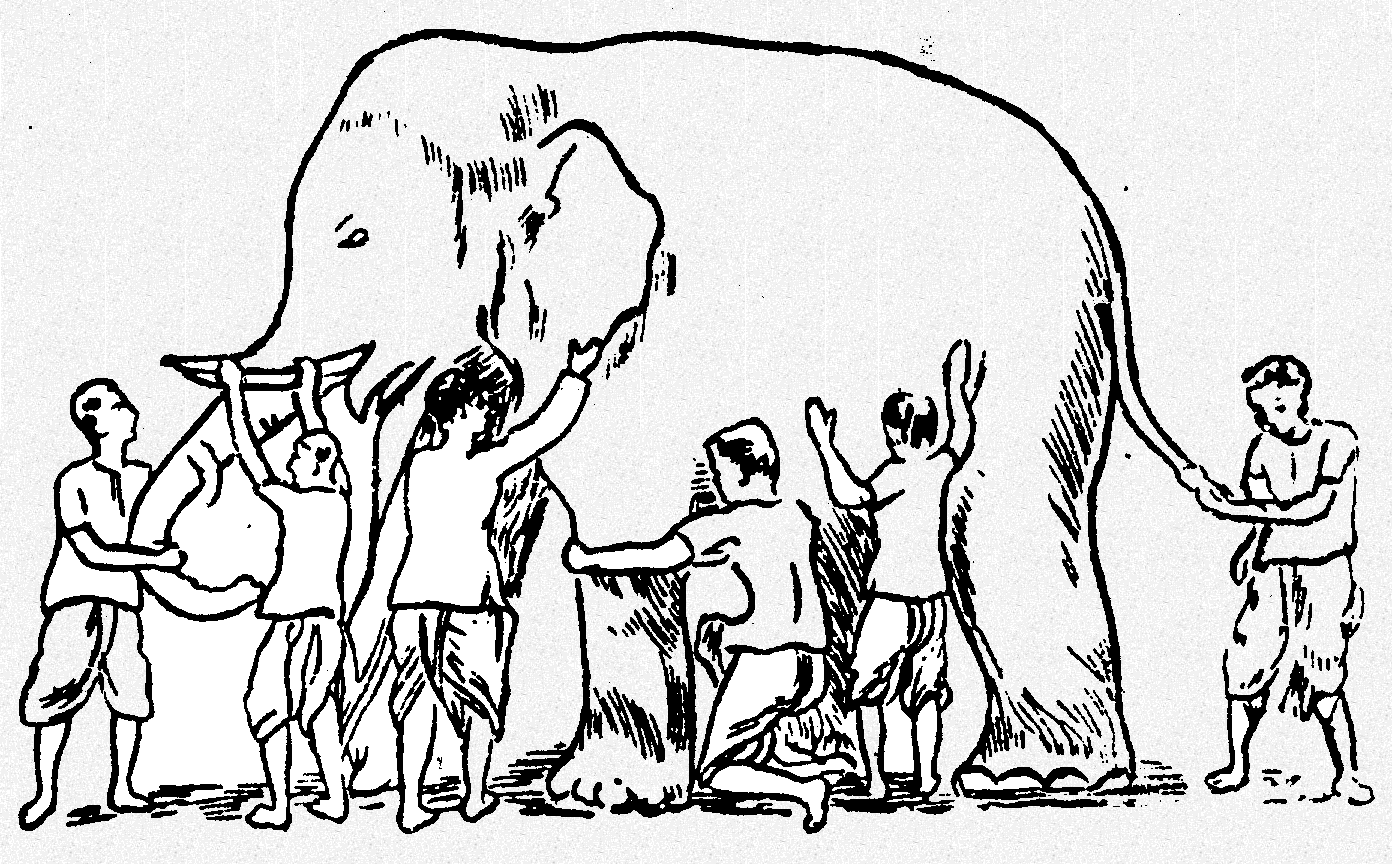
\includegraphics[width=0.99\textwidth]{elephant}
    \caption {\emph{``It's not anything''}}
  \end{columns}
\end{figure}
\end{frame}


\begin{frame}[plain]
\textbf{Philosophy begins with scepticism}\newline
The burden of being convinced of anything universal and not physically demonstrable lies with the other \vspace{10mm}

\textbf{The mental is not necessarily the spiritual}\newline
The sense of eternal life, God and religion is the spiritual, the mental is that I think \vspace{10mm}

\textbf{The mental is represented by the brain state}\newline
All my activity has corresponding neuronal activity, therefore the latter is the exhaustive explanation of the former \vspace{10mm}
\end{frame}



\begin{frame}[plain]
\begin{figure}
  \centering
  \begin{columns}
    \column{0.99\textwidth}
    \centering
    
\includegraphics[width=0.7\textwidth]{tarzan}
    \caption {\emph{``Difference in degree, not kind''}}
  \end{columns}
\end{figure}
\end{frame}


\begin{frame}[plain]
\textbf{If matter can be divided, what is wave-particle duality?}\newline
The lack of understanding of what matter is may indeed happen to encompass the spiritual \vspace{10mm}

\textbf{couldn't there be a third way between matter and spirit}\newline
What assurance is there that the two are mutually exclusive and both are exhaustive of reality? \vspace{10mm}

\textbf{behaviour is explicable at a neurological, habitual, environmental level}\newline
What makes up decisions, however free them seem, is fully accounted for in a determined way \vspace{10mm}
\end{frame}


\begin{frame}[plain]
\begin{figure}
  \centering
  \begin{columns}
    \column{0.99\textwidth}
    \centering
    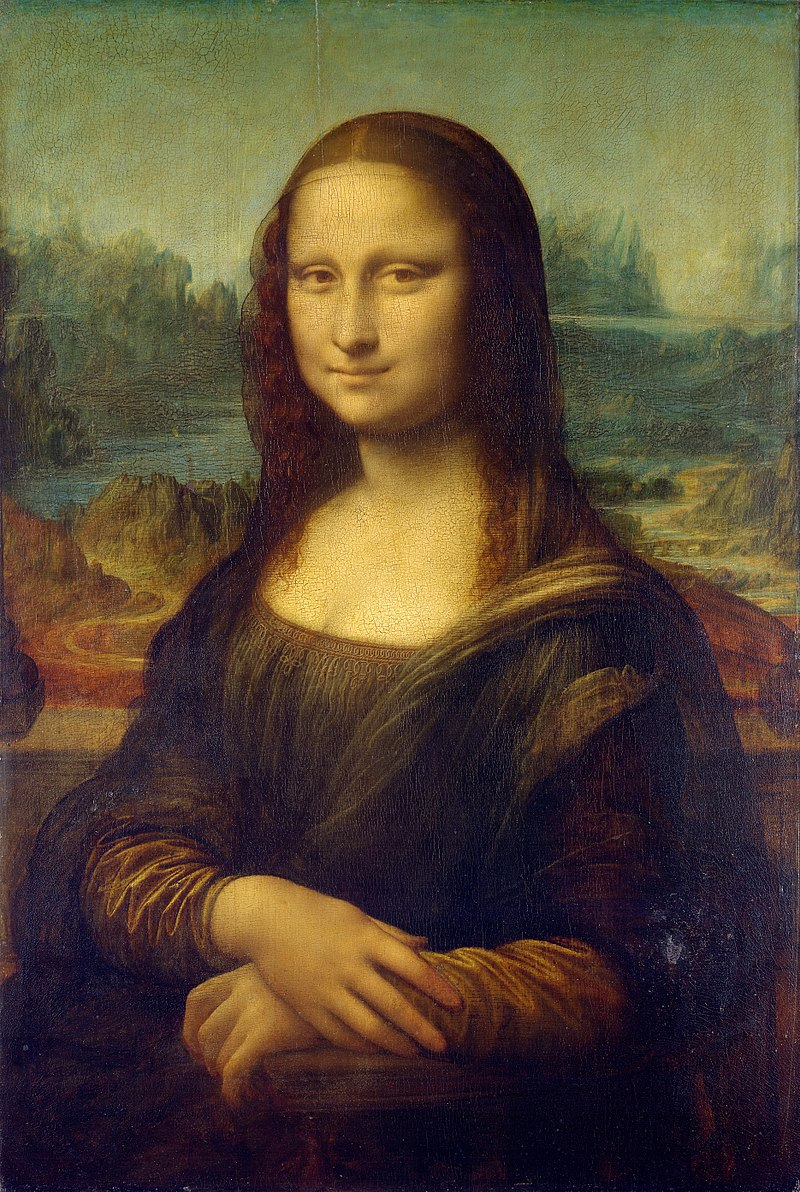
\includegraphics[width=0.7\textwidth,trim=0 150mm 0 0, clip]{mona-lisa}
    \caption {\emph{``Recursive representation''}}
  \end{columns}
\end{figure}
\end{frame}


\begin{frame}[plain]
\textbf{Intelligence is algorithmic}\newline
Advancement of `artificial intelligence' is such that in matters of communication there is no way to distinguish man from mechanism \vspace{10mm}

\textbf{Thought is imagination, memory and fantasy}\newline
A concept is always conceived in a particular way, therefore there is no such thing as a concept as something universal \vspace{10mm}

\textbf{That you seem to understand me suffices}\newline
Language is simply convention, it has no dependence on the immaterial. just like other animals \vspace{10mm}
\end{frame}


\begin{frame}[plain]
\begin{figure}
  \centering
  \begin{columns}
    \column{0.99\textwidth}
    \centering
    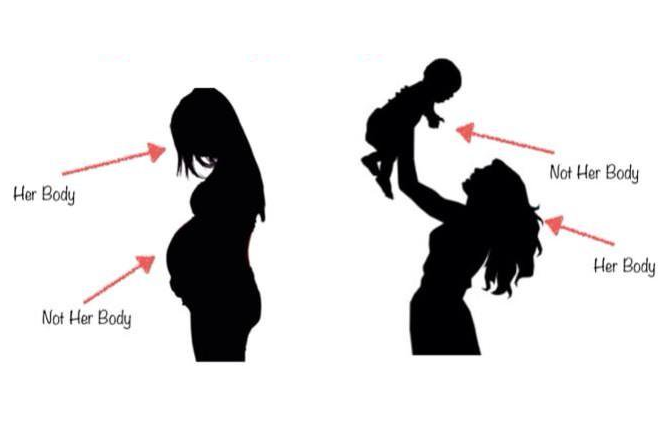
\includegraphics[width=0.99\textwidth,trim=0 0 0 0, clip]{pregnancy}
    \caption {\emph{``\st{My body} Our bodies, my choice''}}
  \end{columns}
\end{figure}
\end{frame}


\begin{frame}[plain]
\textbf{Some happy form of utility seems to work}\newline
happiness is a self defined pursuit and, whilst subject to tension, seeks social harmony \vspace{10mm}

\textbf{I do things for different reasons}\newline
multiplicity in the sources of personal intentionality can be coherently maintained \vspace{10mm}

\textbf{The good is according to decision, not nature}\newline
the good is a virtue whose pursuit is according to the \emph{via media} \vspace{10mm}
\end{frame}


\begin{frame}[plain]
\begin{figure}
  \centering
  \begin{columns}
    \column{0.99\textwidth}
    \centering
    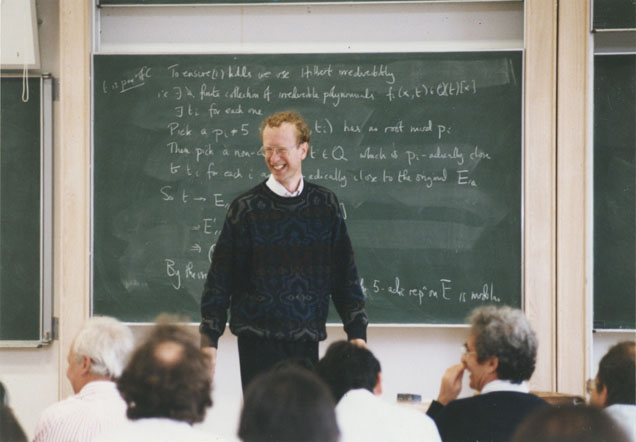
\includegraphics[width=0.99\textwidth,trim=0 0 0 0, clip]{fermats-theorem}
    \caption {\emph{``Mathematics is certain''}}
  \end{columns}
\end{figure}
\end{frame}


\begin{frame}[plain]
\textbf{Truth is not obtained from trust}\newline
Religion is a concept, and has no mechanism by which it can be verified \vspace{10mm}

\textbf{Cleverness is a prerequisite for belief}\newline
What if conclusions of the intellect do not agree with the articles of faith? \vspace{10mm}

\textbf{The contraries have been argued ever since}\newline
Whatever you say, someone else could probably offer a convincing argument to the contrary \vspace{10mm}
\end{frame}


\begin{frame}[plain]
\begin{figure}
  \centering
  \begin{columns}
    \column{0.99\textwidth}
    \centering
    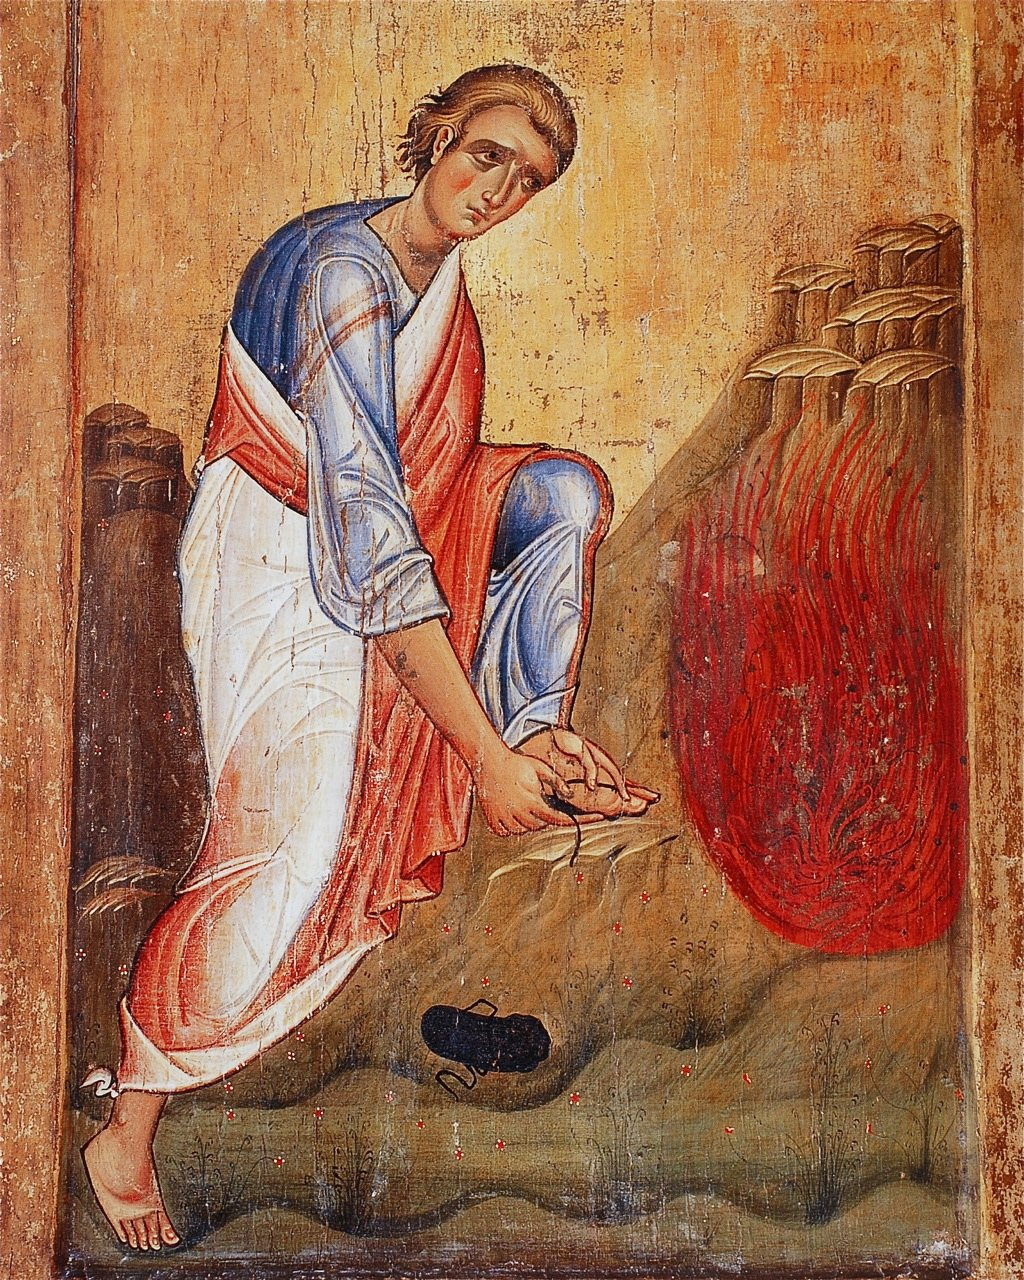
\includegraphics[width=0.7\textwidth,trim=0 100mm 0 0, clip]{burning-bush}
    \caption {\emph{``God said to Moses, `I am who I am'"} Ex 3:14}
  \end{columns}
\end{figure}
\end{frame}


\begin{frame}[plain]
\textbf{The Unmoved Mover is not the Triune God}\newline
The philosophical God is not the Catholic God; what is missing in the former may imply a radically different God with respect to the latter \vspace{10mm}
\end{frame}

\end{document}
